\documentclass{beamer}

% \usepackage{beamerthemesplit} // Activate for custom appearance

\usepackage{multicol}
\usepackage{lmodern}
\usepackage{lipsum}
\usepackage{marvosym}

\title{Augmented approximate Riemann solvers for the shallow water equations with varying bathymetry}
\author{Jacob Ortega-Gingrich\\ Xin Chen}
\date{\today}

\begin{document}

\frame{\titlepage}


\section[Outline]{}
\frame{\frametitle{Outline} \tableofcontents}

\section{Introduction}
\subsection{The shallow water equations}

\frame
{
 \frametitle{The shallow water equations}
 The shallow water equations are given by
 \begin{align*}
h_t+(h u)_x&=0\\
(h u)_t+\left(h u^2+\frac{1}{2} g h^2\right)_x&=-g h b_x
\end{align*}
where $h(x,t)$ is the depth of the water (from the free surface to the sea floor), $u(x,t)$ is the velocity of the water and $b(x)$ is the fixed underwater topography.
}

\frame
{
\frametitle{Some desired properties of the Riemann solver for modeling drying and inundation}
\begin{itemize}
\item<1-> Preservation of depth Non-Negativity of solutions.
\item<2-> Prevention of non-physical oscillations along steep interfaces of shorelines.
\item<3-> Preservation of Steady States. \\
Since tsunami waves are small perturbations of an ocean at rest over variable bathymetry, it is critical that the Riemann solver be able to preserve steady states involving a flat surface even with large variations in the underlying topography.
\end{itemize}
}

\subsection{The wave propagation algorithm}
\frame
{
  \frametitle{The  wave propagation algorithm}
  \begin{itemize}
  \item<1-> The first order method
  \begin{align*}
Q_i^{n+1}&=Q_i^n-\frac{\Delta t}{\Delta x} (\mathcal{A}^+\Delta Q_{i-\frac{1}{2}}^n+\mathcal{A}^-\Delta Q_{i+\frac{1}{2}}^n).
\end{align*}
Where the jump is decomposed into separate waves
\begin{align*}
Q_i^n-Q_{i-1}^n=\sum_{p=1}^{M_w} \mathcal{W}_{i-\frac{1}{2}}^p
\end{align*}
which propagate from the discontinuity at speeds $s_{i-\frac{1}{2}}^p$.  The fluctuations then used to update the cell values are
\begin{align*}
\mathcal{A}^- \Delta Q_{i-\frac{1}{2}}&=\sum_{\lbrace p:s^p_{i-\frac{1}{2}}<0\rbrace} s_{i-\frac{1}{2}}^p \mathcal{W}_{i-\frac{1}{2}}^p\\
\mathcal{A}^+\Delta Q_{i-\frac{1}{2}}&=\sum_{\lbrace p: s_{i-\frac{1}{2}}^p>0\rbrace} s_{i-\frac{1}{2}}^p \mathcal{W}_{i-\frac{1}{2}}^p.
\end{align*}
  \end{itemize}
}

\subsection{The f-wave method}
\frame
{
\frametitle{The f-wave method}
The f-wave method decomposes the jump in the flux instead of the actual cell average, thus the name.
\begin{align*}
f(Q_i)-f(Q_{i-1})=\sum_{p=1}^{M_w} \mathcal{Z}_{i-\frac{1}{2}}^p
\end{align*}
and we may define our updating fluctuations as
\begin{align*}
\label{fwave fluc}
\mathcal{A}^- \Delta Q_{i-1/2}=\sum_{\{p:s_{i-1/2}^p <0\}} \mathcal{Z}_{i-1/2}^p\\
\mathcal{A}^+ \Delta Q_{i-1/2}=\sum_{\{p:s_{i-1/2}^p >0\}} \mathcal{Z}_{i-1/2}^p
\end{align*}
}

\subsection{The Roe solver}
\frame
{
\frametitle{The Roe solver}
It is an approximate Riemann solver based on a linearization about a specific mean state $(\bar h, \hat u)$ where $\bar h$ is the arithmetic mean of the depths on either side of the interface and the speed is given by
\begin{equation}
\label{uhat}
\hat u=\frac{\sqrt{h_{i-1}} u_{i-1}+\sqrt{h_i} u_i}{\sqrt{h_{i-1}}+\sqrt{h_i}}.
\end{equation}
The eigenvalues (known as the Roe wave speeds) of the linearized Jacobian $\hat A$ are $\hat \lambda^1=\hat u-\hat c$, $\hat \lambda^2=\hat u+\hat c$ where $\hat c=\sqrt{g \bar h}$.  The corresponding eigenvectors are
\begin{equation}
\label{roeeig}
\hat r^1=\left(\begin{array}{cc}1\\ \hat u-\hat c\end{array}\right), \hat r^2=\left(\begin{array}{cc} 1\\ \hat u +\hat c\end{array}\right).
\end{equation}
}

\section{The HLLE solver and depth non-negativity}
\frame{
\frametitle{The HLLE solver and depth non-negativity}
\begin{itemize}
\item<1-> For SWE problem, the HLLE solver is a modified version of the Roe solver.
\item<2-> The wave speeds (Einfeldt speeds) are given by
\begin{equation*}
\label{einfeldt}
\check s^1_{i-\frac{1}{2}}= \min(\lambda^-(Q_{i-1}^n),\hat \lambda^-_{i-\frac{1}{2}}), ~~
\check s^2_{i-\frac{1}{2}}=\max(\lambda^+(Q_i^n),\hat \lambda^+_{i-\frac{1}{2}})
\end{equation*}
\item<3-> The corresponding waves are given by $w_{i-\frac{1}{2}}^p=(1,\check s_{i-\frac{1}{2}}^p)^T$
\item<4-> Fails to capture large transonic rarefactions and does not preserve steady states with variable topography.
\end{itemize}
}

\frame
{
\frametitle{transonic rarefaction}
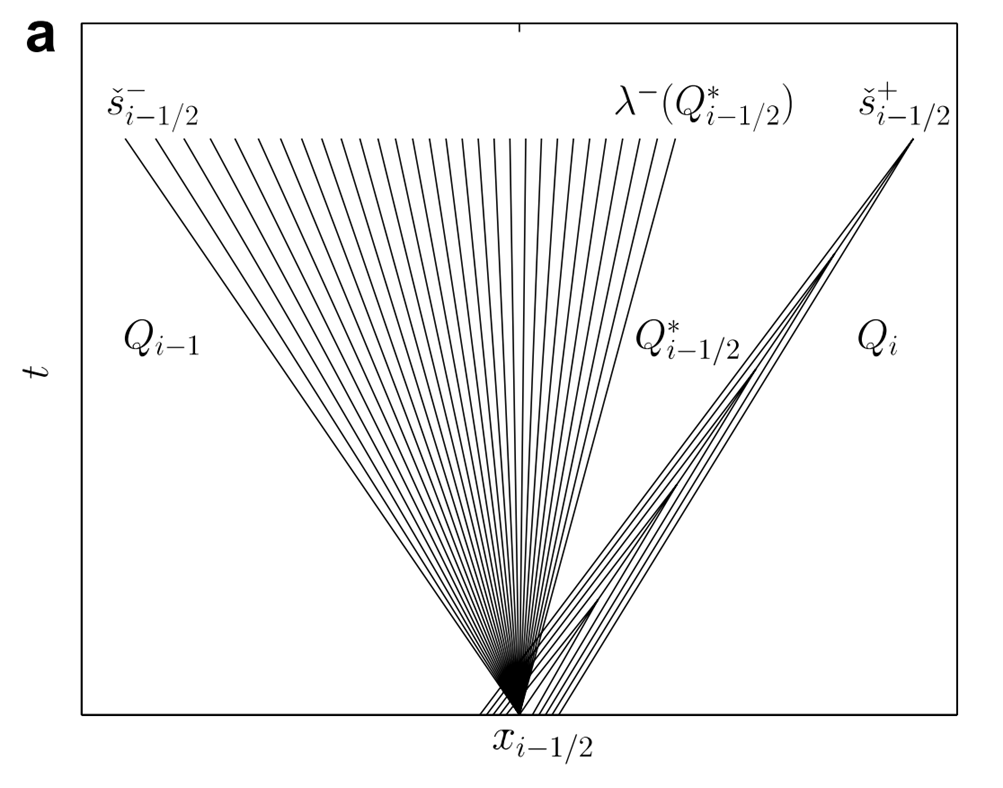
\includegraphics[width=0.83\linewidth]{transonic.png}
}

\section{The augmented solver}
\subsection{The augmented solver for homogeneous SWE}
\frame
{
\frametitle{The augmented solver for homogeneous SWE}
\begin{itemize}
\item<1-> Decomposing the jump into three waves
\begin{align*}
\begin{bmatrix}
H_i-H_{i-1}\\
HU_i-HU_{i-1}\\
\varphi(Q_i)-\varphi(Q_{i-1})
\end{bmatrix}=\sum_{p=1}^3 \alpha_{i-1/2}^p w_{i-1/2}^p.
\end{align*}
Where $\varphi=h u^2+\frac{1}{2} g h^2$ is the momentum flux.
\item<2-> 
The flux waves are defined as
\begin{align*}
\mathcal{Z}_{i-1/2}^p =\left[\mathbf{0}_{2\times1} \quad \mathbf{I}_{2\times2}\right] \alpha_{i-1/2}^p w_{i-1/2}^p
\end{align*}
\item<3-> Update cell averages just like f-wave method
\end{itemize}
}

\frame
{
\frametitle{Determining the basis waves $w_{i-\frac{1}{2}}^p$}
\begin{itemize}
\item<1-> To maintain non-negativity, we choose to include the Einfeldt speeds $\check s_{i-\frac{1}{2}^\pm}$ and their corresponding  in our wave decomposition
\begin{align*}
\left\{ w_{i-1/2}^1,s_{i-1/2}^1\right\}=\left\{\left(1,\check{s}_{i-1/2}^-,\left(\check{s}_{i-1/2}^-\right)^2\right)^T, \check{s}_{i-1/2}^- \right\} \\
\left\{ w_{i-1/2}^3,s_{i-1/2}^3\right\}=\left\{\left(1,\check{s}_{i-1/2}^+,\left(\check{s}_{i-1/2}^+\right)^2\right)^T, \check{s}_{i-1/2}^+ \right\}.
\end{align*}
\item<2-> Choice of "corrector" wave
\begin{align*}
\left\{ w_{i-1/2}^2,s_{i-1/2}^2      \right\}=\left\{  \left(0,0,1\right)^T, \frac{1}{2} \left(\check{s}_{i-1/2}^- + \check{s}_{i-1/2}^+ \right)    \right\},
\end{align*}
\end{itemize}
}

\subsection{The augmented solver for SWE with a source term}
\frame
{
\frametitle{The augmented solver for SWE with a source term}
\begin{itemize}
\item<1-> One more component is added to the decomposition to account for the impact of the source term
\begin{align*}
\begin{bmatrix}
H_i-H_{i-1}\\
HU_i-HU_{i-1}\\
\varphi(Q_i)-\varphi(Q_{i-1}) \\
B_i-B_{i-1}
\end{bmatrix}=\sum_{p=0}^3 \alpha_{i-1/2}^p w_{i-1/2}^p,
\end{align*}
\item<2->  Flux waves are given by
\begin{align*}
\mathcal{Z}_{i-1/2}^p =\left[\mathbf{0}_{2\times1} \quad \mathbf{I}_{2\times2} \quad \mathbf{0}_{2\times1}\right] \alpha_{i-1/2}^p w_{i-1/2}^p
\end{align*}
\end{itemize}
}

\frame
{
\frametitle{Determining $w_0$}
From Theorem 1 in George 2008, steady states must satisfy
\begin{equation}
\tilde{q}(x_r,t)-\tilde{q}(x_l,t)=(b(x_r)-b(x_l))\begin{bmatrix}
\frac{g\bar{H}(q(x_l,t),q(x_r,t))}{\overline{\lambda^+ \lambda^-}(q(x_l,t),q(x_r,t))}\\
0\\
-g\tilde{H}(q(x_l,t),q(x_r,t))\\
1
\end{bmatrix}
\end{equation}
where
\begin{align*}
\overline{\lambda^+ \lambda^-}(q(x_l,t),q(x_r,t))&=\left(\frac{u_l+u_r}{2}\right)^2-g\left(\frac{h_l+h_r}{2}\right)  \\
\bar{H}(q(x_l,t),q(x_r,t))&=\frac{h_l+h_r}{2}\\
\widetilde{\lambda^+ \lambda^-}(q(x_l,t),q(x_r,t))&= \max (0,u_r u_l)-g\left(\frac{h_l+h_r}{2}\right)\\
\tilde{H}(q(x_l,t),q(x_r,t))&=\bar{H}(q(x_l,t),q(x_r,t)) \frac{\widetilde{\lambda^+ \lambda^-}(q(x_l,t),q(x_r,t))}{\overline{\lambda^+ \lambda^-}(q(x_l,t),q(x_r,t))}.
\end{align*}
}

\frame
{
\begin{itemize}
\item<1-> $w_{i-1/2}^0$ must capture the jump in steady states precisely and we choose
\begin{equation}
w_{i-1/2}^0=\begin{bmatrix}
\frac{g\bar{H}(Q_{i-1},Q_i)}{\overline{\lambda^+ \lambda^-}(Q_{i-1},Q_i)}\\
0\\
-g\tilde{H}(Q_{i-1},Q_i)\\
1
\end{bmatrix},\quad s_{i-1/2}^0=0
\end{equation}
\item<2-> We use this new steady state wave along with the same waves from the previous Riemann solver:
\begin{align*}
\left\{ w_{i-1/2}^1,s_{i-1/2}^1\right\}=\left\{\left(1,\check{s}_{i-1/2}^-,\left(\check{s}_{i-1/2}^-\right)^2,0\right)^T, \check{s}_{i-1/2}^- \right\} \\
\left\{ w_{i-1/2}^3,s_{i-1/2}^3\right\}=\left\{\left(1,\check{s}_{i-1/2}^+,\left(\check{s}_{i-1/2}^+\right)^2,0\right)^T, \check{s}_{i-1/2}^+ \right\}\\
\left\{ w_{i-1/2}^2,s_{i-1/2}^2      \right\}=\left\{  \left(0,0,1,0\right)^T, \frac{1}{2} \left(\check{s}_{i-1/2}^- + \check{s}_{i-1/2}^+\right)    \right\}.
\end{align*}
\end{itemize}
}

\frame
{\frametitle{Practical considerations for problems involving dry cells and shorelines}
\begin{itemize}
\item Treatment for near-dry cells
\begin{itemize}
\item When the depth of the cell is positive but very close to zero, numerical difficulties occur. Therefore, we consider cells with a depth smaller than a certain threshold a dry cell and set the depth and momentum to zero. In the simulation, the threshold is set to $10^{-3}$ meters.
\end{itemize}
\item Treatment for neighboring wet and dry cells
\item Treatment for steep shorelines
\item Treatment for transonic rarefaction waves
\end{itemize}
}


\frame
{
\frametitle{Treatment for neighboring wet and dry cells}
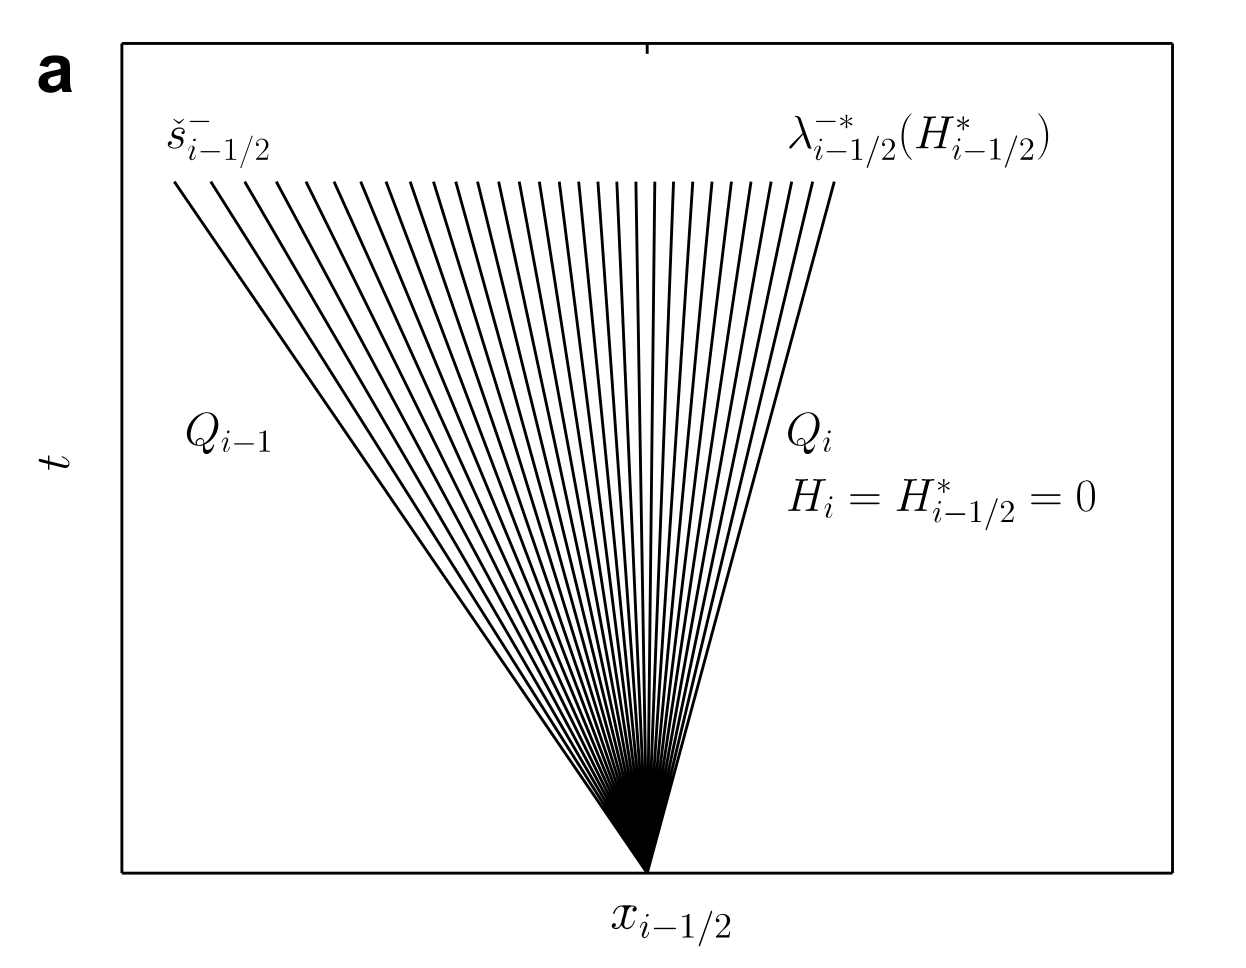
\includegraphics[width=0.83\linewidth]{wetanddry.png}
\begin{align*}
\check s_{i-\frac{1}{2}}^-=U_{i-1}-\sqrt{g H_{i-1}}, ~~~ \check s_{i-\frac{1}{2}}^+=U_{i-1}+2\sqrt{g H_{i-1}}
\end{align*}
}

\frame
{
\frametitle{Treatment for steep shorelines}
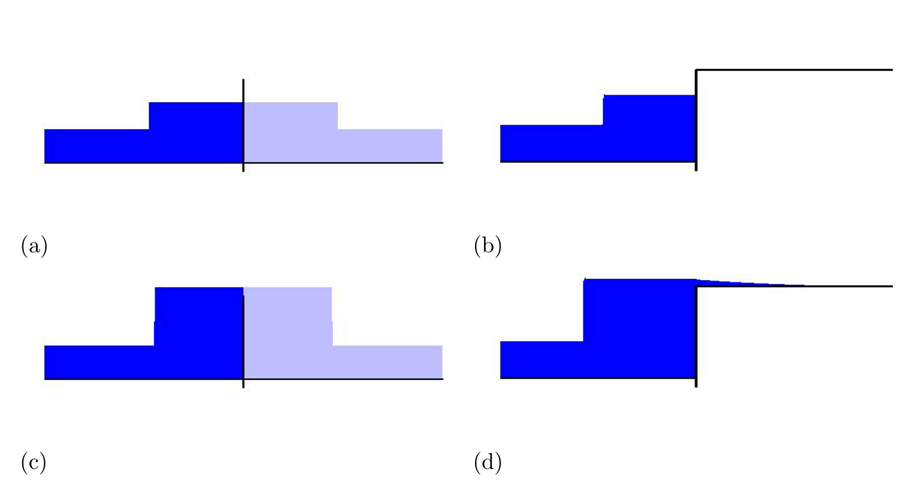
\includegraphics[width=0.83\linewidth]{steep.png}
\begin{equation}
\check{H}^*=\frac{HU_{L}-HU_R+\check{s}_{i-1/2}^+ H_R-\check{s}_{i-1/2}^- H_L}{\check{s}_{i-1/2}^+-\check{s}_{i-1/2}^-}
\end{equation}
}

\frame
{
\frametitle{Treatment for transonic rarefaction waves}
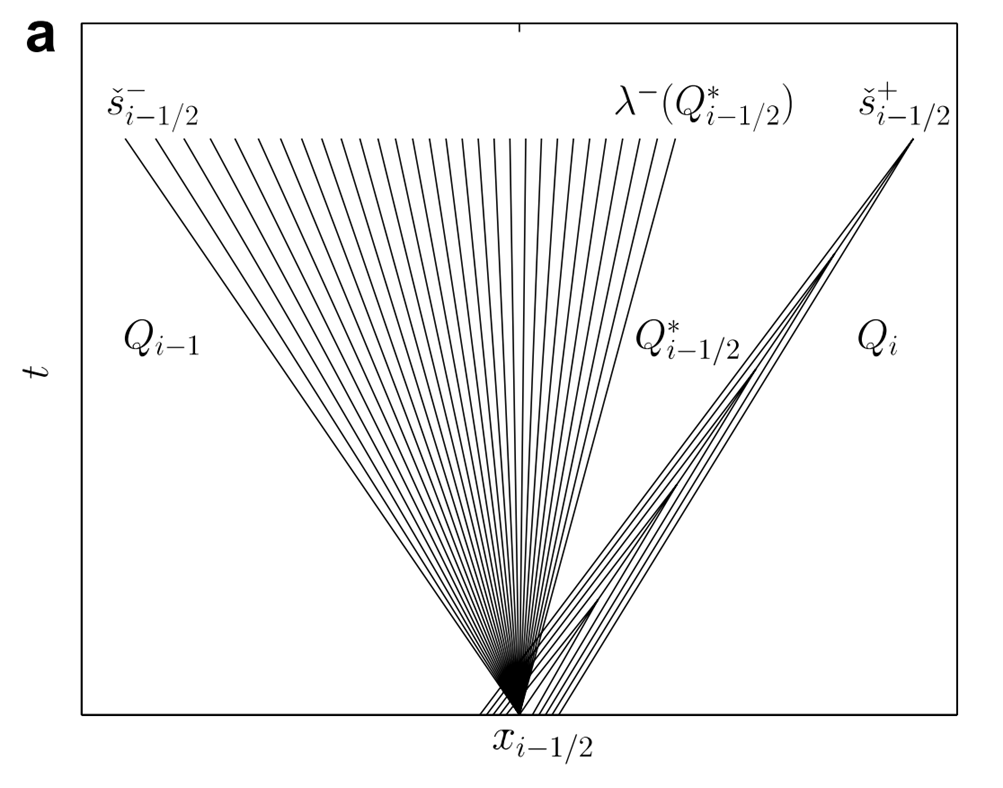
\includegraphics[width=0.83\linewidth]{transonic.png}
\begin{align*}
\lbrace w_{i-\frac{1}{2}}^2,s_{i-\frac{1}{2}}^2 \rbrace=\lbrace
(1,\lambda_{i-\frac{1}{2}}^{-*}(H_{i-\frac{1}{2}}^*),(\lambda_{i-\frac{1}{2}}^{-*}(H_{i-\frac{1}{2}}^*))^2,0), \lambda_{i-\frac{1}{2}}^{+*}(H_{i-\frac{1}{2}}^*)
\rbrace.
\end{align*}
}



\section{Numerical Experiments}
\frame
{
\frametitle{Numerical Experiments}
\href{run:./beach.mp4}{Numerical simulation of beach problem}
\begin{columns}[t]
\column{.5\textwidth}
\centering
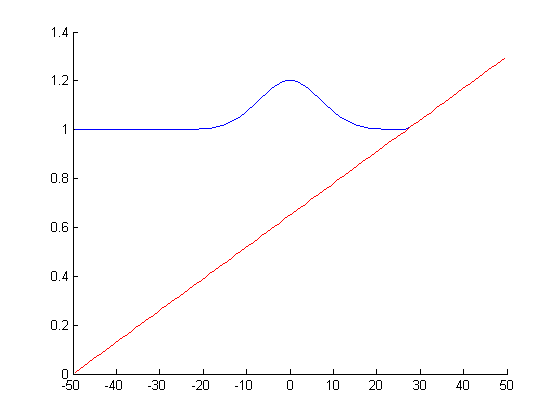
\includegraphics[width=5cm,height=3.5cm]{beach1.png}\\
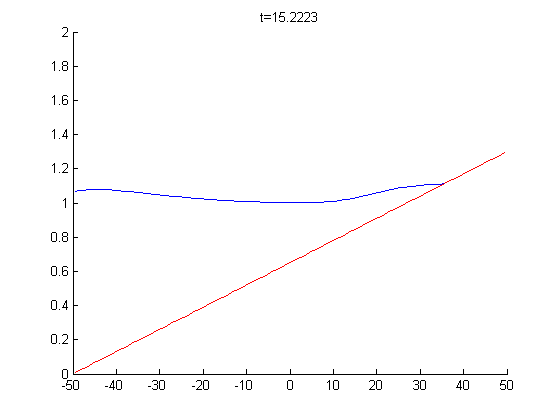
\includegraphics[width=5cm,height=4cm]{beach2.png}
\column{.5\textwidth}
\centering
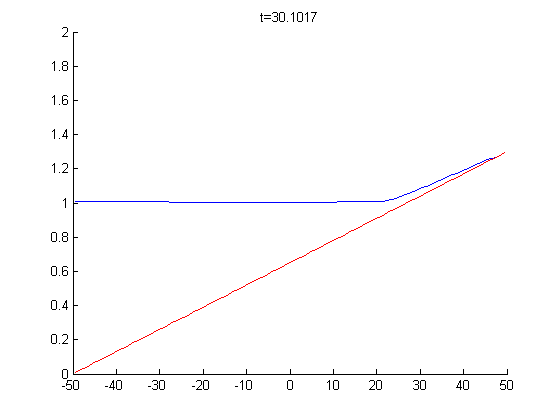
\includegraphics[width=5cm,height=4cm]{beach3.png}\\
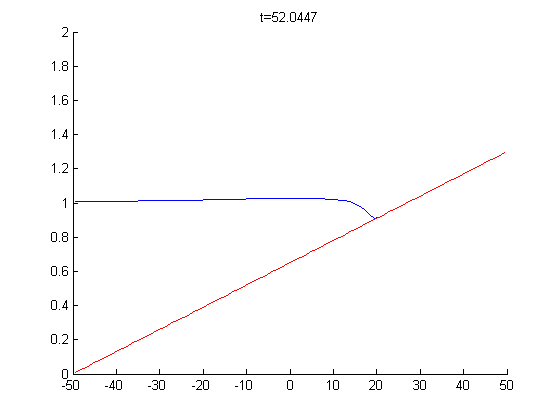
\includegraphics[width=5cm,height=4cm]{beach4.png}
\end{columns}
}
\frame
{
\frametitle{Numerical Experiments}
\href{run:./dambreak.mp4}{Numerical simulation of dambreak problem}
\begin{columns}[t]
\column{.5\textwidth}
\centering
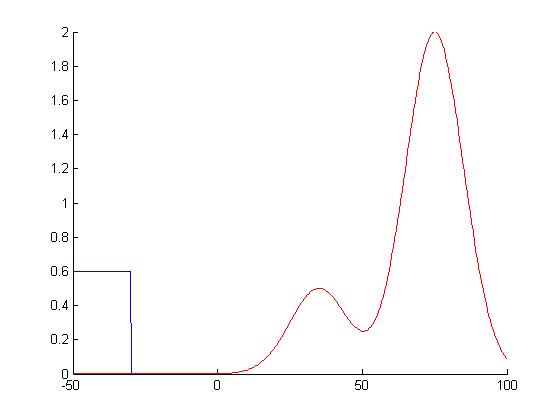
\includegraphics[width=5cm,height=3.5cm]{valley1.png}\\
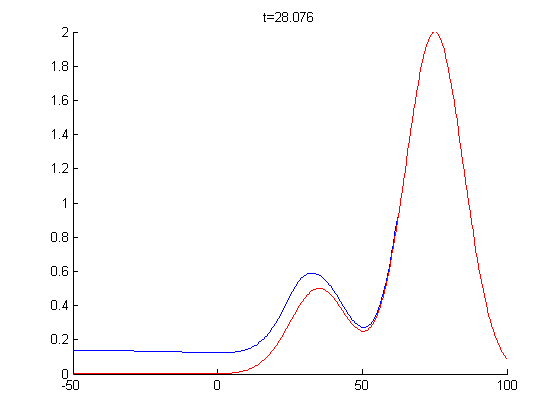
\includegraphics[width=5cm,height=4cm]{valley2.png}
\column{.5\textwidth}
\centering
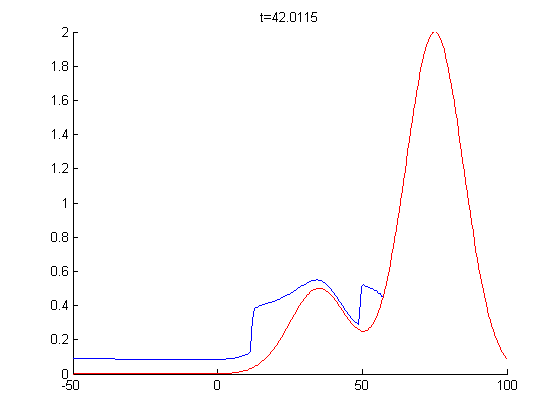
\includegraphics[width=5cm,height=4cm]{valley3.png}\\
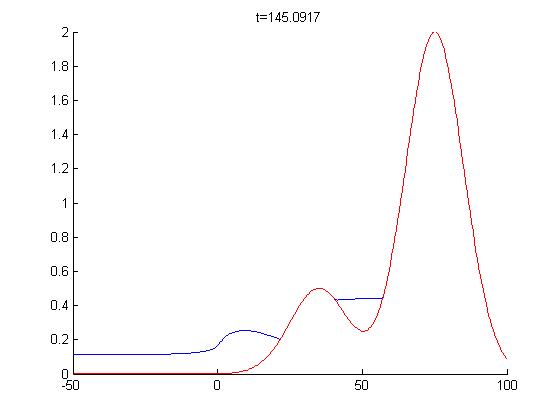
\includegraphics[width=5cm,height=4cm]{valley4.png}
\end{columns}
}

\section{Summary}
\frame
{\frametitle{Summary}
Thus, we have described a method which:
\begin{itemize}
\item is well-balanced
\item is "mostly" depth positive semi-definite
\item can handle neighboring wet and dry cells including cases involving steep shorelines
\item provides a natural entropy fix for dealing with transonic rarefaction.
\end{itemize}
}

\section{References}
\frame
{
\begin{thebibliography}{1}

\bibitem{GeorgePhD} D.L. George, Finite Volume Methods and Adaptive Refinement for Tsunami Propagation and Inundation, Ph.D. Thesis, University of Washington, Seattle, WA, 2006

\bibitem{George} D.L. George, Augmented Riemann solvers for the shallow water equations over variable topography with steady states and inundation, Journal of Computational Physics, 227 (2008)  3089-3113.

\bibitem{FVM} R.J. LeVeque, Finite Volume Methods for Hyperbolic Problems.  Texts in Applied Mathematics, Cambridge University Press, Cambridge, 2002.

\end{thebibliography}
}

\end{document}
